La première des alertes que nous proposons de traiter est l'alerte
dite du \emph{Grand Veymont,} issue de l'enregistrement d'un appel au
secours effectué par un accompagnateur en montagne, au sujet d'un de
ses clients.
%
Cette alerte est la plus simple est la plus courte de celles que nous
traiterons ici.

\subsection{Présentation de l'alerte}
\label{subsec:9-2-1}

L'alerte du \emph{Grand Veymont} est l'extrait, d'une durée de 1
minute 06, d'un appel effectué par un accompagnateur en montagne au
sujet d'un de ses clients \autoref{anx:retrans-gv-verb}.


Cette alerte est la plus courte de celles que nous présenterons ici,
elle est composée de 12 extraits, pour un total de 16 expressions.



Pas d'objets multiples

les indications données par le requérant sont assez précises et
détaillées, il est donc possible de définir une \emph{zone initiale de
  recherche} de petite taille. Nous avons défini une \ac{zir} de
\SI{25}{\kilo\meter\squared} (\autoref{fig:zir_grand_veyont}).

\begin{figure}
  \centering
  \begin{tikzpicture}
  \tikzset{et/.style={above,font=\footnotesize\vphantom{Ag}}}
  %
  \node[inner sep=0pt, anchor=south west] (image) at (0,0){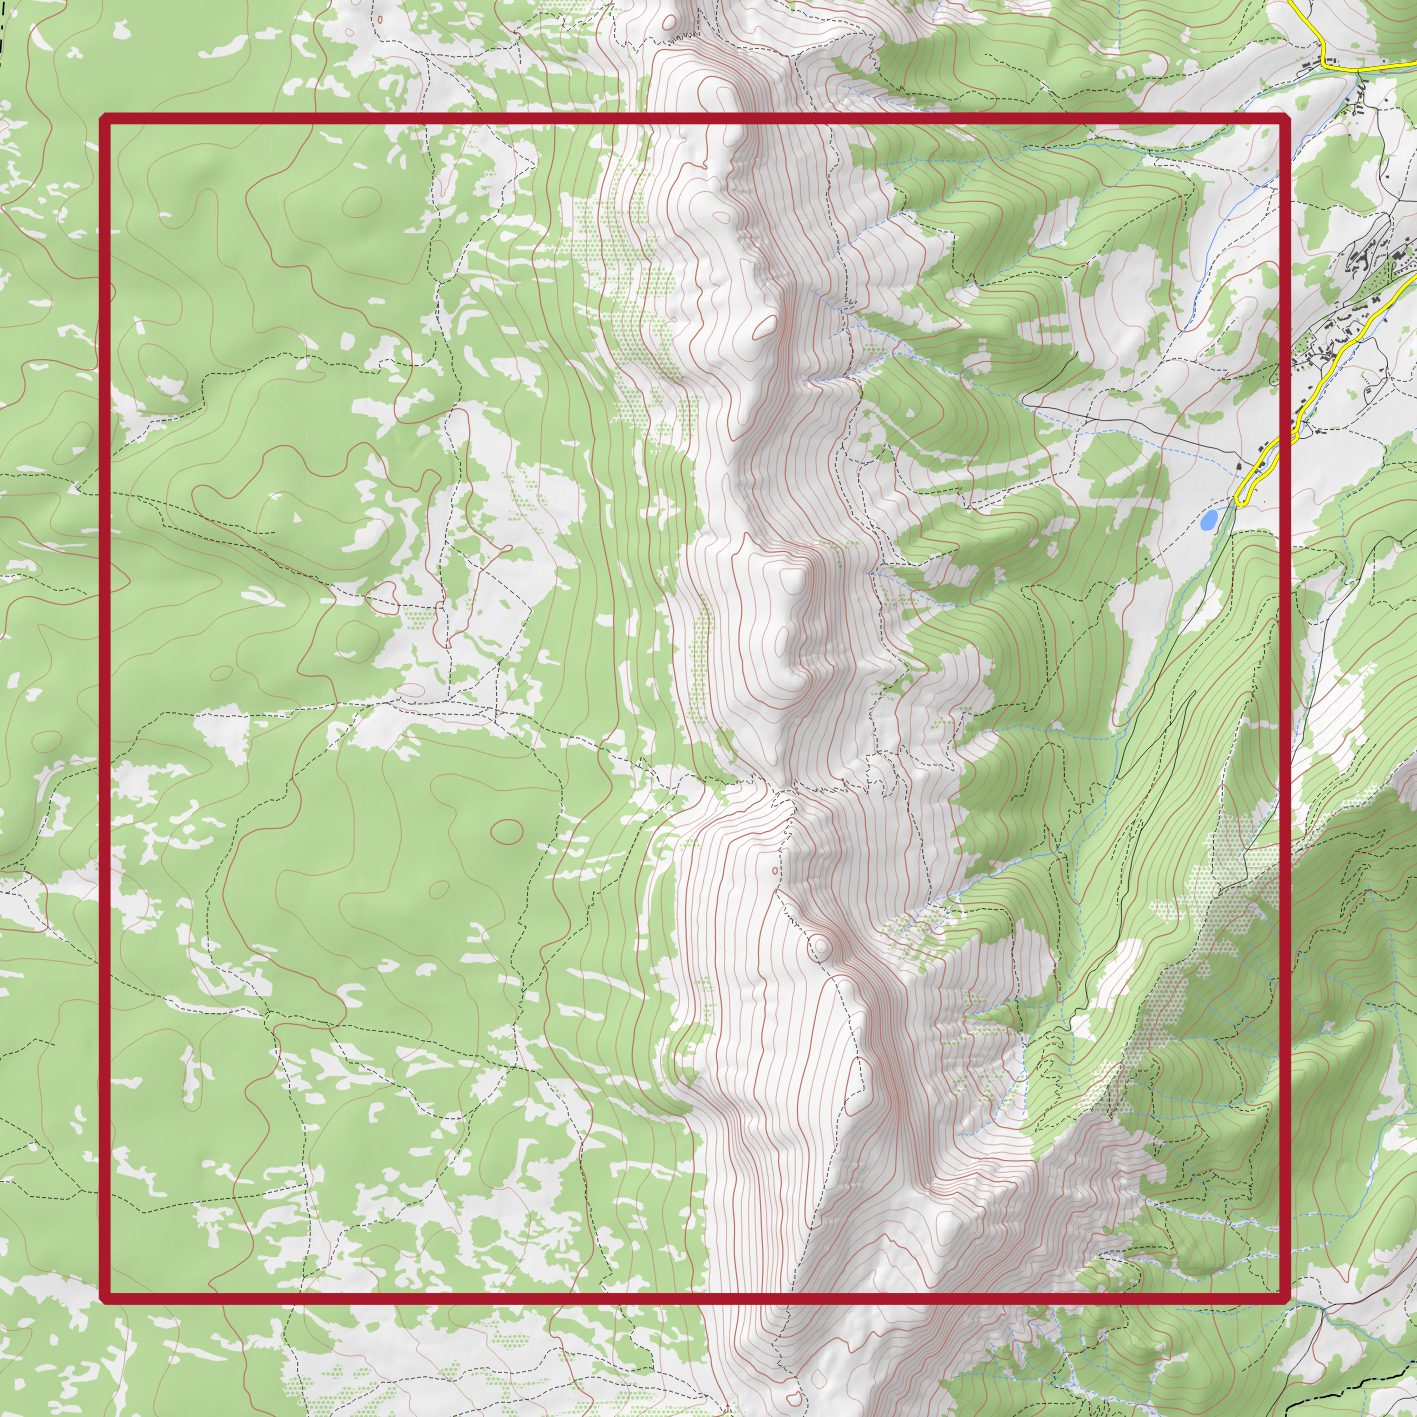
\includegraphics{./figures/ZIR_grand_veymont.png}};
  %
  \begin{scope}
    \node (P2) at ([yshift=-.5cm]image.south east) {};
    \node (P1) at ([yshift=-.5cm]image.south west) {};
    %
    \foreach \x [evaluate=\xshift using \x/10, evaluate=\rad using (\x * .0004) + .01] in {0,...,100}
    {
      \draw[fill=black,draw=none, below] ([xshift=\xshift cm, yshift=-.5cm]P1) circle [radius=\rad cm];
    }
    %
    \path(P1 |- 0cm,-1cm) --++ (10,0)
    node[et,pos=0] {0}
    node[et,pos=.1] {0,1}
    node[et,pos=.2] {0,2}
    node[et,pos=.3] {0,3}
    node[et,pos=.4] {0,4}
    node[et,pos=.65] {0,65}
    node[et,pos=1] {1};
    % Échelle
    \draw[-] (P2 |- -1cm,-1cm) --++ (-1,0) node[et,pos=.5] {\SI{500}{\meter}};
    % Légende détaillée
    \path (P1) -- (P2) node[pos=.5, yshift=-1cm] {\tiny Pour la légende détaillée du fond topographique voir \autoref{anx:topo_leg}. Sources: BD TOPO 2018, BD ALTI 2018.}; 
  \end{scope}
\end{tikzpicture}
  \caption{Zone initiale de recherche pour l'alerte \enquote{Grand Veymont}}
  \label{fig:zir_grand_veyont}
\end{figure}


\subsubsection{Retranscription et identification des indices de localisation}
\label{subsec:9-2-1-1}


Le verbatim de l'enregistrement audio de l'alerte \emph{Grand Veymont}
est donné dans la \autoref{anx:retrans-gv-verb}.
%
Comme nous l’expliquions dans le \autoref{chap:05}, 


Une partie des indices retranscrits ne sont cependant pas pertinents
pour notre cas d'appliqaution.

% Entre Grand Veymont et pas de la ville
% Je ne suis pas sur le sommet
% Je suis sous le grand Veymont
% Côté Sud/Nord

% Au dela

% not foret

% 800
Enfin, les deux derniers extraits, nous renseignent sur la distance
euclidienne qui sépare actuellement le requérant et la victime du Pas
de la Ville, qui est d'environ 800 mètres.
%
\begin{dialogue}
  \Sec \direct{11-1} Vous êtes à combien du Pas de la ville ?
  % 
  \Req \direct{12-1} \textins{À} 800 mètres, je crois, à vol d'oiseau
\end{dialogue}

Ce type de configuration est représenté par la relation de
localisation
\onto[orl]{Distance\-Quanti\-ta\-ti\-ve\-Planimetrique}. Comme nous
l'indiquions dans le \autoref{chap:07}, cette relation de localisation
est atomique, elle n'admet donc pas de décomposition.


\begin{figure}
  \centering
  \begin{tikzpicture}[scale=.7]
  \def\decalageX{-.2}
  \def\decalageY{-.2}
  % Courbe
  \begin{scope}[transparency group]
    % fond
    \begin{scope}
      \path[ffa]  (3,0) -- (4.5, 2) -- (6,0) -- cycle;
    \end{scope}
    % bords
    \begin{scope}
      \path[ffc] (1,.8) -- (3.6,.8) -- (4.5, 2) -- (5.4,.8) -- (8,.8) ;
      \path[ffc_fade_m] (0,.8) -- (1,.8) ;
      \path[ffc_fade] (8,.8) -- (9,.8) ;
    \end{scope}
  \end{scope}
  % Axes X, Y
  \begin{scope}
    % Axe X
    \begin{scope}
      % Axe
      \draw[<->] (0, \decalageX) --++ (9, 0) coordinate (x axis);
      % Graduations
      \foreach \n/\t in {0.5/{},1.5/{},2.5/{400},3.5/{},4.5/{800},5.5/{},6.5/{1200},7.5/{},8.5/{}}
      {
        \draw[-] (\n, \decalageX - .05) --++ (0, .1);
        \node[below, font=\footnotesize] at (\n, \decalageX - .05) {\t};
      }
      % label
      \node[below left, yshift=-.1cm, font=\small] at (x axis)
      {\itshape Distance \normalfont (m)};
    \end{scope}
    % Axe Y
    \begin{scope}
      % Axe
      \draw[-] (\decalageY ,0) --++ (0, 2) coordinate (y axis);
      % Graduations
      \foreach \n/\t in {0/{0},2/{1}}
      {
        \draw[-] (\decalageY -.05, \n) --++ (.1, 0);
        \node[left, font=\footnotesize] at (\decalageY -.05, \n) {\t};
      }
      % Label
      \node[above] at (y axis) {$\mu$};
    \end{scope}
  \end{scope}
  \begin{scope}
    % Seuil 1
    \draw[ffc,line width=.5] (3,\decalageY) -- (3,0);
    \draw[fill, RdBu-9-1] (3,\decalageY) circle (2pt);
    \draw[fill, RdBu-9-1] (3,0) circle (2pt);
    % Seuil 2
    \draw[ffc,line width=.5] (4.5,\decalageY) -- (4.5,2);
    \draw[fill, RdBu-9-1] (4.5,\decalageY) circle (2pt);
    \draw[fill, RdBu-9-1] (4.5,2) circle (2pt);
    % Seuil 3
    \draw[ffc,line width=.5] (6,\decalageY) -- (6,0);
    \draw[fill, RdBu-9-1] (6,\decalageY) circle (2pt);
    \draw[fill, RdBu-9-1] (6,0) circle (2pt);
  \end{scope}
\end{tikzpicture}

  \caption{XXXX \enquote{Grand Veymont}}
  \label{fig:fuzzy_veyont_distance}
\end{figure}


\subsection{Modélisation de l'alerte}
\label{subsec:9-2-2}


\subsubsection{Au-delà du Pas de la Ville}

La spatialisation de l'indice de localisation \enquote{je suis au-delà
  du Pas de la Ville}, pose certaines difficultés.

La relation de localisation de cet indice est représentée par le
concept \onto[orl]{Après\-Jalon\-Sut\-Itineraire}
(\autoref{anx:orl_dic})

\subsubsection{À 800 mètres du Pas de la Ville}

Ce dernier indice de localisation ne présente pas de difficultés
spécifiques pour être mis en place.





\subsubsection{Fusion des zones de localisation compatibles}

À la suite de la spatialisation des différents indices de localisation
et de la composition des 

\subsection{Critique de la modélisation}
\label{subsec:9-2-3}

\tdi{Impact de la position du toponyme "pas de la ville" sur la
  modélisation}

Un autre problème notable est l'impact que peut avoir la géométrie des
objets de référence sur le résultat de la spatialisation. Par exemple,
l'indice de localisation : \enquote{À \SI{800}{\meter} du Pas de la
  Ville} a été spatialisé en calculant la métrique
\onto[orla]{Distance} à partir du ponctuel plaçant l'oronyme
\enquote{Pas de la Ville} dans la base de données. Or, la
représentation d'un géotype étendu, comme un pas ou une crête, par un
point est une approximation conséquente, impactant fortement la
spatialisation.


%%% Local Variables:
%%% mode: latex
%%% TeX-master: "../../../../main"
%%% End:
